\section{Python Exercise: Image Scaling with Separable Filters}\label{sec:p7}

Figure \ref{fig:p7} shows the results of the four pre-filters. Since the visual difference is subtle, their corresponding MSEs are included. Method (a) and (c) are actually the same since $h = \delta$ so their MSEs are the same. The pattern (around leg and scarf area) of method (b) is overly smoothed.

\begin{figure}[htbp]
	\centering
	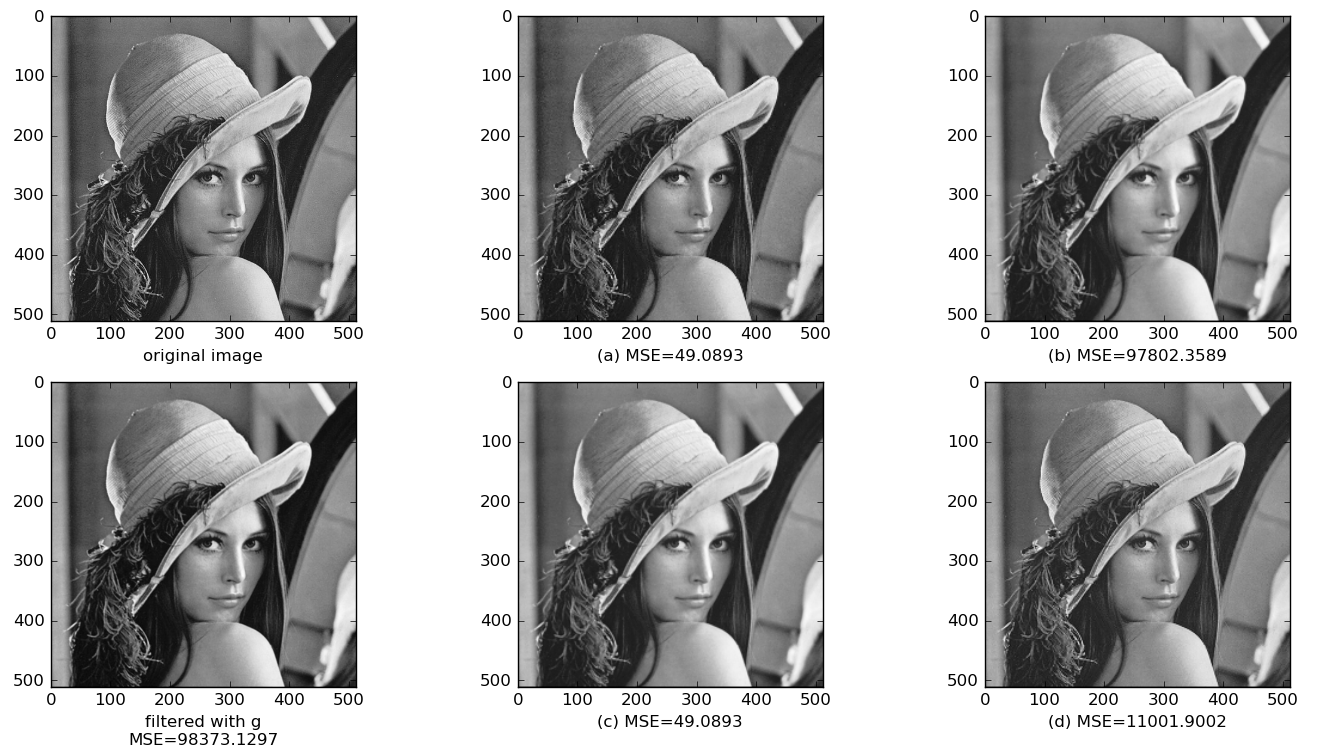
\includegraphics[width=\textwidth]{images/p7}
	\caption{Original image and four pre-filters (a-d) with corresponding MSE}
	\label{fig:p7}
\end{figure}